\documentclass[10pt,oneside,slovak,a4paper]{article}

\usepackage[slovak]{babel}
%\usepackage[T1]{fontenc}
\usepackage[IL2]{fontenc}
\usepackage[utf8]{inputenc}
\usepackage{graphicx}
\usepackage{url} % príkaz \url na formátovanie URL
\usepackage{hyperref} % odkazy v texte budú aktívne (pri niektorých triedach dokumentov spôsobuje posun textu)

\usepackage{cite}
\usepackage{indentfirst}
%\usepackage{times}
%\usepackage{fancyhdr}
%\usepackage{csquotes} Uvodozvky    \enquote{TEXT}

%Nastavenie cesty pre obrazky
\graphicspath{ {./images/} }

\pagestyle{myheadings}%{headings} {fancy} zmiznu nazvy sekcii
%\fancyhf{}
%\fancyhead[LE, RO]{\leftmark} LEFT EVEN, RIGHT ODD
%\fancyhead[RE, LO]{\thepage}
\title{Aplikácie a riešenia dištančného vzdelávania a e-vzdelávania\thanks{Semestrálny projekt v predmete Metódy inžinierskej práce, ak. rok 2020/21, vedenie: Ing. Fedor Lehocki, PhD.}}

\author{Lukáš Štrbo\\[2pt]
	{\small Slovenská technická univerzita v Bratislave}\\
	{\small Fakulta informatiky a informačných technológií}\\
	{\small \texttt{xstrbol@stuba.sk}}
	}

\date{\small 12. december 2020}



\begin{document}

\maketitle

\begin{abstract}
E-vzdelávanie sa stáva stále viac populárnejšou metódou nadobúdania vedomostí. Mnohí ľudia ju preferujú najmä kvôli rýchlosti a efektívnosti získavania poznatkov.
Prostredníctvom internetu sa dokážeme vzdelávať pomocou rôznych aplikácií, webov, kurzov alebo aj diskusných fór.
S e-vzdelávaním ide ruka v ruke dištančné vzdelávanie, ktoré hlavne v ťažších časoch, ako je napríklad nemožnosť zúčastňovať sa prezenčnej výučby z dôvodu pandémie COVID-19, 
 je voľbou číslo jedna. V tejto práci si zadefinujeme pojmy e-vzdelávanie a dištančné vzdelávanie. Cieľom tejto práce je sprehľadniť čitateľovi rôzne typy dištančného vzdelávania. Rozoberieme si a porovnáme riešenia dištančného vzdelávania a ich priamu
 aplikáciu. Zameriame sa na výhody a nevýhody, ale aj ktoré softvéry alebo platformy sú lepšie pre dištančné vzdelávanie na základe výskumu a akým výzvam čelia školy počas pandémie COVID-19.
\end{abstract}

%\tableofcontents

\section*{Úvod} %Nezobrazi sa cislovanie
\label{uvod}
%Uvod do problematiky
Vzdelávanie prostredníctvom počítača a webu je stále viac populárnejšou metódou výučby, či ide o školy alebo o samoukov. V súvislosti aj s celosvetovou pandémiou 
COVID-19 bola väčšina škôl nútená prejsť na dištančné vzdelávanie. Dištančné vzdelávanie je spojené s e-vzdelávaním. Tieto výrazy špecifikujeme v sekcii \ref{rozdiely}.  
Nie vždy je jasné, čo sa pod dištančnou výučbou myslí a aké technológie pod ňu spadajú. Preto v sekcii \ref{typy} a \ref{Vyvojsys} budeme bližšie špecifikovať, čo
pod dištančným vzdelávaním rozumieme a aký vývoj mali rôzne podporné systémy.
 
V súvislosti s pandémiou COVID-19 a prechodom na dištančné vzdelávanie prichádzajú aj určité výzvy vo vzdelávaní.
Je veľmi dôležité zabezpečiť kontinuitu vzdelávania aj počas pandémie a nemožnosti prezenčnej výučby.
V rámci tohto prechodu bol vykonaný výskum zameraný na spätnú väzbu od študentov k spokojnosti, výhodám, nevýhodám a on-line riešeniam vzdelávania.

\section{Definícia dištančného vzdelávania a e-vzdelávania}
\label{rozdiely}
Dištančné vzdelávanie je proces výučby, ktorý prebieha na diaľku bez priameho kontaktu učiteľa a študenta.\cite{India}.
Dištančné vzdelávanie zahŕňa poskytovanie elektronických alebo iných systémov na nadviazanie a udržiavanie komunikácie medzi učiteľmi a študentmi.
Stará koncepcia dištančného vzdelávania bola spojená výlučne s tlačenými materiálmi, zatiaľ čo nová koncepcia dištančného vzdelávania zahŕňa materiály používané prostredníctvom netlačených médií, ako sú počítače, nahrané prednášky vo formáte videí alebo aj interaktívne stretnutia medzi študentmi.

Existujú 2 typy dištančného vzdelávania na základe interakcie študentov, a to synchrónne a asynchrónne.
Synchrónna metóda vyžaduje prezenčnú účasť študenta.
Asynchrónna metóda nevyžaduje prezenčnú účasť.

E-vzdelávanie je závislé od technológii, podporuje a zlepšuje výučbu. Ide o elektronickú technológiu na poskytovanie, podporu a zdokonaľovanie výučby a učenia sa. 

E-vzdelávanie je prirodzene vhodné na dištančné a flexibilné vzdelávanie, ale dá sa použiť aj v spojení s prezenčnou výučbou \cite{elearningDef}.
V prípade spojenia s prezenčnou výučbou sa používa termín blended learning. 
E-vzdelávanie môže tiež odkazovať na vzdelávacie webové stránky, ako napríklad webové stránky ponúkajúce pracovné listy a interaktívne cvičenia.


\section{Typy dištančnej výučby}
\label{typy}
%Uvod do typov distancnej vyucby
Dištančná výučba môže nadobúdať rôzne formy. Postupom času sa rozvíjali rôzne typy sprostredkovania dištančnej výučby. Typy dištančnej výučby môžeme rozdeliť podľa použitia
špecifických technológií a ich kombináciou s prezenčnou výučbou \cite{WiktorzakKotowski}.

Rozdelenie podľa použitia špecifických technológií:
\begin{itemize}
	\item \textbf{Technology-based training (TBT)} alebo aj e-vzdelávenie.
	\item \textbf{Computer-based training (CBT)}, ktorý používa počítače v procese výučby na prenos znalostí, vykonávanie cvičení alebo simulácii. V rámci tohto konceptu sú aj rôzne kurzy, ktoré v minulosti boli dodávané na CD.
	\item \textbf{Web-based training (WBT)} je typ dištančnej výučby, ktorý prebieha na internete prostredníctvom protokolu TCP/IP. Zahŕňa prenos znalostí, ako aj ich overenie, komunikáciu medzi používateľmi a riadením vzdelávacieho procesu s využitím webových stránok a webových aplikácií.
\end{itemize}

Rozdelenie podľa kombinácie technológií s prezenčnou výučbou:
\begin{itemize}
	\item \textbf{Instructor-led training (ILT)} je výučbový proces, v ktorom učiteľ vyučuje skupinu študentov väčšinou priamo v priestoroch školy. Výučba môže nadobudnúť aj takú formu, počas ktorej učiteľ komunikuje so žiakmi prostredníctvom internetu.
	\item \textbf{Synchronous learning (SL)} znamená, že výučba je realizovaná prostredníctvom internetu. Študenti aj učitelia sú prihlásení do virtuálneho učebného priestoru, v ktorom prebieha výučba.
	\item \textbf{Blended learning (BL)} alebo aj hybridné vyučovanie je spôsob výučby, ktorý vznikol kombináciou tradičnej a dištančnej formy výučby. V tomto modeli výučby sú konzultácie a prednášky prednášané väčšinou on-line, zatiaľ čo cvičenia a praktické hodiny sa uskutočňujú prezenčnou formou.
\end{itemize}


\begin{figure}[h]
	\centering
	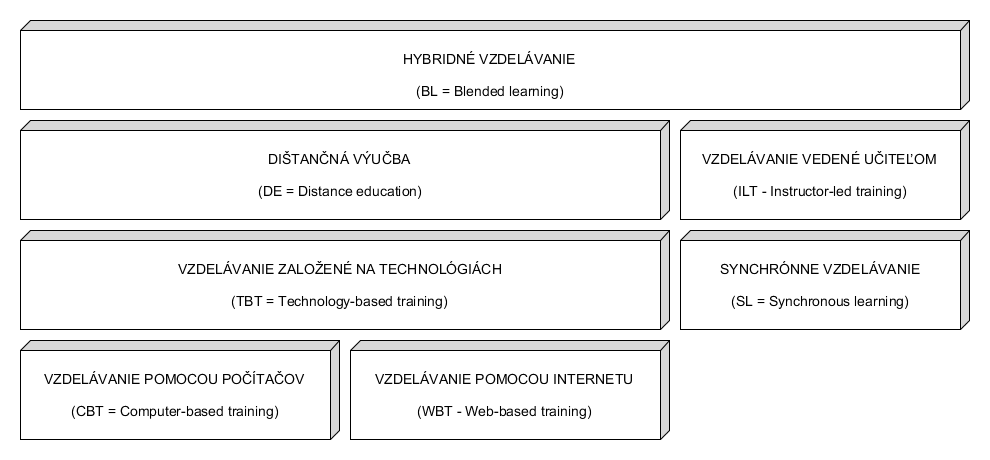
\includegraphics[width=\textwidth]{Vztahy_DE.png}
	\caption{Vzťahy medzi pojmami v dištančnom vzdelávaní\cite{WiktorzakKotowski}}
	\label{Vztahy_medzi_pojmami}
\end{figure}

%Referencia na obrazok
Vzťahy medzi pojmami spojenými s dištančným vzdelávaním sú znázornené na obrázku \ref{Vztahy_medzi_pojmami}.%obrazok 1 alebo obrazok Č. 1
Oblasť dištančného vzdelávania pokrýva širokú sféru technológií a metód vzdelávania.
V závislosti od prenášaného obsahu sa používajú rôzne nástroje a techniky výučby.

\section{Vývoj podporných systémov pre dištančné vzdelávanie}
\label{Vyvojsys}
Systémy podporujúce dištančné vzdelávanie boli pôvodne navrhnuté na výučbu pomocou počítača (CBT)\cite{WiktorzakKotowski}.

S príchodom internetu sa objavilo veľa nástrojov, ktoré podporujú vzdelávanie prostredníctvom webu (WBT).
Pôvodne išlo len o statické stránky, ktoré poskytovali učebné materiály.
Neskôr sa objavili dynamické stránky, ktoré vyžadovali určitú interakciu používateľov, ako sú napríklad diskusné fóra alebo interaktívne cvičenia.
Ide o internetové služby, ktoré spolupracujú s databázou obsahujúcou učebné materiály a testy na kontrolu vedomostí študentov.
Takéto služby umožňujú učenie a komunikáciu v asynchrónnom režime. Učebné materiály môže učiteľ priebežne aktualizovať a ukladať do elektronickej databázy.
Priama komunikácia medzi študentom a učiteľom je nadviazaná aj vďaka e-mailu.

Ďalším krokom vo vývoji systémov na podporu dištančného vzdelávania bol vznik synchrónnych komunikačných nástrojov, ako sú chat, audio a videokonferencie, virtuálna tabuľa a zdieľanie obrazovky.
Spojenie týchto komunikačných nástrojov do aplikácie funguje ako virtuálna učebňa.
Dnes sú to napríklad Google Classroom, Google Meet, Cisco Webex Meetings, Zoom Meetings, Microsoft Teams a podobne.
Vývoj podporných systémov je zobrazený na obrázku \ref{Vyvoj_podp_sys_DE}.

\begin{figure}[h]
	\centering
	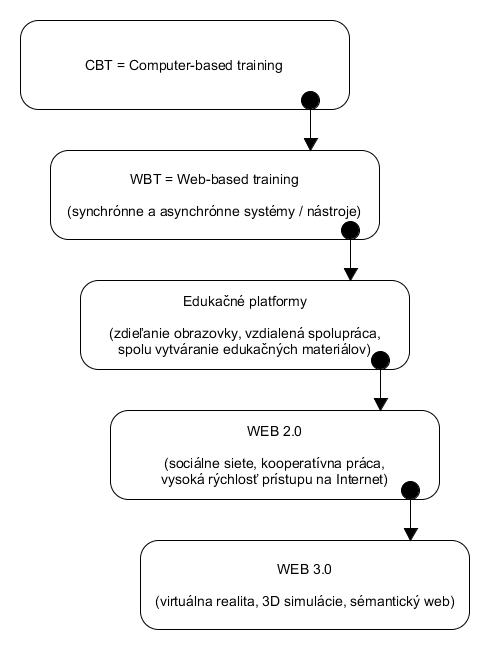
\includegraphics[scale=0.15, height=100mm,width=0.6\textwidth]{Dev_Of_SupSys_DE.jpg}
	\caption{Vývoj podporných systémov pre dištančné vzdelávanie\cite{WiktorzakKotowski}}
	\label{Vyvoj_podp_sys_DE}
\end{figure}

\section{Výhody a nevýhody dištančnej výučby}
V nasledujúcich podsekciách si rozoberieme výhody a nevýhody dištančného vzdelávania\cite{Sokolova2018}.
Dištančné vzdelávanie nesie so sebou veľa pozitívnych aspektov, ktoré pomahajú nielen študentom, ale aj učiteľom a univerzitám.
Avšak dištančné vzdelávanie prináša aj isté negatíva, ako napríklad formu testovania, komunikácia a interakcia študentov s učiteľmi a podobne. 

\subsection{Výhody}
Výhodou študovania na diaľku je, že študent potrebuje iba zariadenie s prístupom na internet, ako napríklad počítač \cite{Sokolova2018}.
Študent sa sám rozhodne, kedy a kde bude učebné materiály študovať. Študenti môžu ušetriť aj peniaze za školné, dopravu, učebnice, skriptá ale aj ubytovanie.
Zároveň sa nesmelí študenti cítia komfortnejšie v kladení otázok učiteľom, ak niečomu nechápu. Študenti majú možnosť si vypočuť prednášku viackrát (napr. videonahrávky prednášok).
Dištančné vzdelávanie takisto umožňuje učiteľom rýchlo získavať spätnú väzbu od veľkého počtu študentov.
Takéto vzdelávanie je ideálnou alternatívou denného štúdia aj pre ľudí so zdravotným postihnutím.
Títo študenti nemajú vždy možnosť fyzicky navštevovať hodiny z dôvodu zlého zdravotného stavu.

\subsection{Nevýhody}
Nevýhodou študovania na diaľku je, že študent je zbavený živej komunikácie s učiteľom a ostatnými študentmi \cite{Sokolova2018}. Prednášky tým strácajú veľa na významovom obsahu.
Nesmelí študenti, ktorí sa cítia lepšie pri interakcii na diaľku, si nezvyknú na živú komunikáciu.
On-line testovanie nie je vhodné na rozvoj schopnosti samostatne myslieť, asimilovať materiál a snažiť sa ho uplatniť vo svojom živote.
Výsledky, ktoré získa študent po zvládnutí daného testu, nebudú vždy odrážať úroveň jeho vedomostí z témy, na ktorú sa pripravoval.
Zároveň dlhodobá práca pri počítači má negatívny vplyv na zdravie, zrak a chrbticu.


\section{Výzvy vo vzdelávaní a výučba počas pandémie COVID-19}
V súvislosti s pandémiou COVID-19 boli školy a univerzity zatvorené a pre zabezpečenie kontinuity vzdelávania, sa z prezenčnej výučby prešlo na on-line výučbu \cite{covid19}.
Sme tak svedkami núteného prerušenia klasickej organizácie vzdelávania, jej štruktúr a rutín. Prioritou všetkých vzdelávacích systémov je neprerušovať výučbu,
a preto sa pokladá za dôležité zabezpečiť výučbu aj v on-line priestore.

Medzi rôzne iniciatívy na oslovenie študentov počas on-line výučby patrí napríklad využívanie špecializovaných platforiem pre on-line výučbu a oficiálnych webových stránok,
ktoré centralizujú iniciatívy v tejto oblasti. Ďalšou iniciatívou je podpora študentov a rodičov prostredníctvom častých správ, vysvetlení, otázok a odpovedí za pomoci používania e-mailu a sociálnych sietí,
ale aj reorganizácia hodnotiacich postupov, ako napríklad úprava alebo zrušenie skúšok, písomiek a testov. Jednou z hlavných iniciatív je zavedenie konkrétnych opatrení zameraných na dosiahnutie rovnosti vo vzdelávaní,
najmä preto, že zraniteľné skupiny sa počas krízových situácií stávajú ešte viac zraniteľnejšími (príkladom je poskytnutie počítačov a telekomunikačných balíkov úradmi pre rodiny v ťažkostiach).  %ktoré uprednostňujú vlády, školy alebo učitelia s cieľom efektívne 

\subsection{Výskum}
Zámerom výskumu bolo zistiť, aké sú najčastejšie používané on-line riešenia, výhody a nevýhody dištančnej výučby a či študentom vyhovuje takýto typ výučby. \cite{covid19} 

Vzorku vo výskume tvorilo 152 študentov z Fakulty psychológie a pedagogických vied Ovídiovej univerzity v Konstanci, ktorá sa nachádza v Rumunsku.
Výskumu sa zúčastnili ženy vo veku od 18 do 52 rokov zo všetkých stupňov štúdia.
Výskum sa uskutočnil on-line prostredníctvom Google formulárov. 

\subsection{Výsledky výskumu}
Výskum tvorilo 8 otázok, z ktorých si rozoberieme nasledujúce 4 otázky \cite{covid19}.

Prvá otázka sa zaoberala názorom študentov ohľadom prechodu z prezenčnej výučby na dištančnú výučbu spôsobeného pandémiou COVID-19.
64.47\% opýtaných odpovedalo, že im dištančná výučba vyhovuje. Pre 34,21\% opýtaných je dištančná výučba prijateľná a 1,31\% opýtaným dištančná výučba nevyhovuje.

Druhá otázka skúmala najpoužívanejšie on-line platformy počas dištančného vzdelávania.
Výsledky ukazujú, že 92,10\% účastníkov a ich učiteľov používa Cisco Webex Meetings, 42,10\% používa WhatsApp a e-mail, 41,44\% Zoom Meetings, 1,31\% Moodle a 1,31\% Academis.
Výsledky druhej otázky sú zobrazené v grafe č. \ref{Graf1} a tabuľke č. \ref{tabulka1}.

Tretia otázka umožnila študentom identifikovať hlavné výhody dištančného vzdelávania.
Výsledky ukazujú, že 45,39\% študentov je spokojných s prístupom k didaktickým prostriedkom, knihám, kurzom a informáciám. 23,68\% je spokojných s flexibilnejším rozvrhom
a 75,57\% je spokojných s možnosťou zúčasťnovať sa hodín bez ohľadu na to, kde sa nachádzajú.

Štvrtá otázka sa týkala identifikácie hlavných nevýhod dištančného vzdelávania. 55,92\% študentov nie je spokojných s veľkým počtom jednotlivých domácich úloh.
27,63\% má ťažkosti s časovým manažmentom, 5,92\% nie je spokojných s kontrolou a hodnotením domácich úloh a 38,15\% študentom chýba živá komunikácia so spolužiakmi a učiteľmi.

\begin{figure}[h]
	\centering
	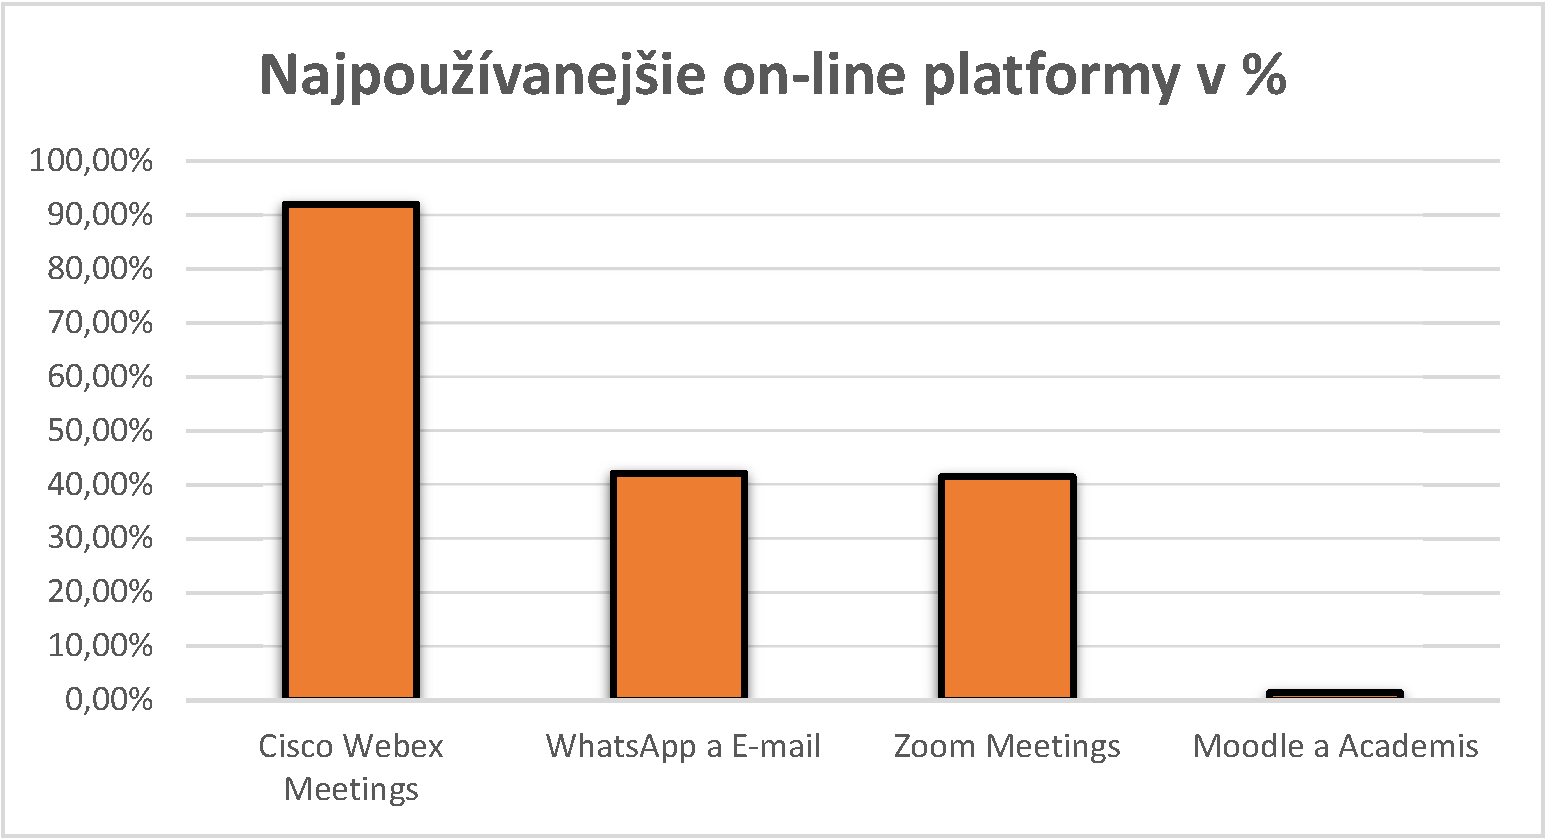
\includegraphics[scale=0.35, width=\textwidth]{GrafOnlineRies.pdf}
	\caption{Najčastejšie používané on-line riešenia podľa výskumu \cite{covid19}.}
	\label{Graf1}
\end{figure}

\begin{table}[h]
	\centering
	\begin{tabular}{|l|l|}
	\hline
	\textbf{Platfomy}    & \textbf{Najpoužívanejšie on-line platformy v \%} \\ \hline
	Cisco Webex Meetings & 92,10 \%                                         \\ \hline
	WhatsApp a E-mail    & 42,10 \%                                         \\ \hline
	Zoom Meetings        & 41,44 \%                                         \\ \hline
	Moodle a Academis    & 1,31 \%                                          \\ \hline
	\end{tabular}
	\caption{Dáta z grafu č.\ref{Graf1} \cite{covid19}}
	\label{tabulka1}
\end{table}

\section*{Záver}
Vývoj podporných systémov sa čoraz viac urýchľuje a prichádza sa aj na ich nové riešenia.
V dnešnej pokročilej dobe a taktiež v rámci technologického pokroku je možné uskutočnovať dištančné vzdelávanie prostredníctvom internetu.

Na margo uzatvárania škôl z dôvodu celosvetovej pandémie COVID-19 boli školy nútené prejsť na dištančné vzdelávanie.
Dištančné vzdelávanie so sebou prináša nielen určité pozitíva, ale aj negatíva. 
Vo výskume boli účastníkmi zodpovedné otázky ohľadom výhod a nevýhod, ale aj prechodu na dištančnú výučbu.
Výskum ukazuje, že iba malé percento opýtaných malo problémy s prechodom na dištančnú formu výučby.
V rámci výskumu môžeme vidieť aj najčastejšie používané on-line platformy pre dištančné vzdelávanie, ktorým konkuruje Cisco Webex Meetings.

\paragraph{Historické súvislosti}
Iba približne pred päťdesiatimi rokmi vznikali prvé komerčné počítače.
Pomocou nich sa nebolo možné efektívne vzdelávať, nakoľko v tej dobe internet nebol tak rozšírený a softvérov bolo málo.
Najprv vznikali kurzy na osobné počítače dodávané na CD. S postupom času a celosvetovým prepojením cez internet vzniklo učenie pomocou vzdelávacích webov.
Na tejto koncepcii je založené aj e-vzdelávanie. S rozvojom internetu a počítačov je tu istá postupnosť vývoja podporných systémov, hlavne pre dištančné vzdelávanie.

\paragraph{Spoločenské súvislosti}
Kvôli celosvetovej pandémii COVID-19 boli ľudia nútení dodržiavať izoláciu od ostatných ľudí.
Študenti, učitelia ale aj školy sa ocitli v situácii, ktorá si vyžadovala prechod na dištančné vzdelávanie.
Prechod nie je jednoduchý ani z hľadiska technického vybavenia študentov či škôl, ale ani z hľadiska komunikácie a náročnosti štúdia. 

\paragraph{Vplyv počítačov na zdravie}
Dištančné vzdelávanie prináša veľa výhod, ale aj nevýhod. Medzi nevýhody v prvom rade patrí vplyv počítačov na zdravie.
Počas pandémie COVID-19 sú študenti a učitelia nútení vykonávať výučbu prostredníctvom internetu.
Dlhodobé sedenie za počítačom a pozeranie sa do obrazovky počítača môže spôsobiť veľké zdravotné problémy.
Práca za počítačom je spojená aj s nedostakom pohybu, čo môže s odstupom rokov viesť až k ťažkým zdravotným problémom, hlavne s chrbticou a zrakom.


\bibliography{zdroje}
\bibliographystyle{plain}
\end{document}
